%%%%%%%%%%%%%%%%%%%%%%%%%%%%%%%%%%%%%%%
% Deedy - One Page Two Column Resume
% LaTeX Template
% Version 1.1 (30/4/2014)
%
% IMPORTANT: THIS TEMPLATE NEEDS TO BE COMPILED WITH XeLaTeX
%
% This template uses several fonts not included with Windows/Linux by
% default. If you get compilation errors saying a font is missing, find the line
% on which the font is used and either change it to a font included with your
% operating system or comment the line out to use the default font.
% 
% CHANGELOG:
% v1.1:
% 1. Fixed several compilation bugs with \renewcommand
% 2. Got Open-source fonts (Windows/Linux support)
% 3. Added Last Updated
% 4. Move Title styling into .sty
% 5. Commented .sty file.

\documentclass[]{deedy-resume-openfont}

\begin{document}

%%%%%%%%%%%%%%%%%%%%%%%%%%%%%%%%%%%%%%
%
%     CURRENT DATE FOR DRAFTS
%
%%%%%%%%%%%%%%%%%%%%%%%%%%%%%%%%%%%%%%
% \lastupdated

%%%%%%%%%%%%%%%%%%%%%%%%%%%%%%%%%%%%%%
%
%     John Hoffer
%
%%%%%%%%%%%%%%%%%%%%%%%%%%%%%%%%%%%%%%

\namesection{John}{Hoffer}{ 
%\urlstyle{same}\url{http://hoff.in} \\
\href{mailto:hof@alumni.harvard.edu}{hof@alumni.harvard.edu} | \href{https://www.linkedin.com/in/john-hoffer-65086aa3/}{LinkedIn}
}

%%%%%%%%%%%%%%%%%%%%%%%%%%%%%%%%%%%%%%
%
%     COLUMN ONE
%
%%%%%%%%%%%%%%%%%%%%%%%%%%%%%%%%%%%%%%

\begin{minipage}[t]{0.33\textwidth} 

%%%%%%%%%%%%%%%%%%%%%%%%%%%%%%%%%%%%%%
%     EDUCATION
%%%%%%%%%%%%%%%%%%%%%%%%%%%%%%%%%%%%%%

\section{Education} 

\subsection{Harvard College}
\location{BA: 2016 | GPA: 3.51}
\descript{Concentration: Neurobiology}
\descript{Secondary: Computer Science}
\sectionsep

% \subsection{Minot High School}
% \location{2012 | Minot, North Dakota}
% \sectionsep

%%%%%%%%%%%%%%%%%%%%%%%%%%%%%%%%%%%%%%
%     SKILLS
%%%%%%%%%%%%%%%%%%%%%%%%%%%%%%%%%%%%%%

\section{Skills}
\subsection{Programming}
\location{Use on daily basis:}
GLSL \textbullet{} Python \textbullet{} Slurm\\ 
JavaScript ( D3 \textbullet{} Node \textbullet{} TypeScript ) \\
\location{Use in past projects:}
C++ \textbullet{} PHP \textbullet{} SQL \textbullet{} MATLAB \textbullet{} \LaTeX\ \\
\location{Learning:}
Lua \textbullet{} Haskell \textbullet{} Wolfram \\
CUDA \textbullet{}  .NET \textbullet{} C\# \\
\location{Daily Workflow:}
Bash \textbullet{} Tmux \textbullet{} Vim \textbullet{} RegEx \\
\sectionsep

\subsection{Design}
\location{Current Projects:}
Blender (Python API) \textbullet{} X3D \textbullet{} CSS \\ 
\location{Frequent Usage:}
3ds Max \textbullet{} Inkscape \textbullet{} Gimp \\
\sectionsep

%%%%%%%%%%%%%%%%%%%%%%%%%%%%%%%%%%%%%%
%     COURSEWORK
%%%%%%%%%%%%%%%%%%%%%%%%%%%%%%%%%%%%%%

\section{Coursework}
\subsection{Computer Science}
Rendering and Image Processing \\
Dynamic \& Stochastic Processes \\
Computer Graphics \\
Visualization \\
\sectionsep

\subsection{Life Science}
Computational Neuroscience \\
Principals of Neuroengineering \\
Computational Cognitive Neuro. \\
Cellular Basis of Neural Function \\
Drug Discovery and Development \\
\sectionsep

%%%%%%%%%%%%%%%%%%%%%%%%%%%%%%%%%%%%%%
%
%     COLUMN TWO
%
%%%%%%%%%%%%%%%%%%%%%%%%%%%%%%%%%%%%%%

\end{minipage} 
\hfill
\begin{minipage}[t]{0.66\textwidth} 

%%%%%%%%%%%%%%%%%%%%%%%%%%%%%%%%%%%%%%
%     EXPERIENCE
%%%%%%%%%%%%%%%%%%%%%%%%%%%%%%%%%%%%%%

\section{Experience}

\runsubsection{Harvard SEAS}
\descript{| Fellow }
\location{February 2016 --- current | Visual Computing Group, Cambridge, MA}
\vspace{\topsep}
\begin{tightemize}
\item Built a pipeline to render ray-tracings from CNN image reconstructions.
\item Wrote a web server to handle terabytes of image data efficiently in real-time
\item Contributed to 5 open source projects
\item Developed several UIs to give the research community real-time collaborative access to neural reconstructions
\item Negotiated deliverable APIs for a multi-million dollar grant
\end{tightemize}
\sectionsep

\runsubsection{Wyss Institute at Harvard}
\descript{| Microfabrication Intern}
\location{February---August 2015 | Human Organs-on-Chips, Boston, MA}
\begin{tightemize}
\item Designed components for development of novel microfluidic cell culture assays
\item Developed and tested improved microscale fabrication procedures
\end{tightemize}
\sectionsep

\runsubsection{Massachusetts General Hospital}
\descript{| Research Intern}
\location{June---August 2013 | Psychiatric Genetics Unit, Boston, MA}
\begin{tightemize}
\item Prepared DNA to correlate cognitive traits with single DNA base pairs
\item Identified possible genes for future study through a literature review
\end{tightemize}
\sectionsep

%%%%%%%%%%%%%%%%%%%%%%%%%%%%%%%%%%%%%%
%     Key Open Source Projects
%%%%%%%%%%%%%%%%%%%%%%%%%%%%%%%%%%%%%%

\section{Key Open Source Projects}
\runsubsection{Neuroglancer}
\location{January 2018 | Google | \href{https://github.com/Rhoana/neuroglancer}{Github Link}}
\begin{tightemize}
\item Designed and developed editing functionality for a Web UI in use by Google, Harvard, Princeton, and Johns Hopkins.
\end{tightemize}
\sectionsep
\runsubsection{OpenSeadragon GL}
\location{January 2017 | OpenSeadragon | \href{https://github.com/thejohnhoffer/viaWebGL}{Github Link}}
\begin{tightemize}
\item Enabled real-time parallel image processing on large-scale images in browser.
\end{tightemize}
\sectionsep

%%%%%%%%%%%%%%%%%%%%%%%%%%%%%%%%%%%%%%
%     JOURNAL PUBLICATIONS
%%%%%%%%%%%%%%%%%%%%%%%%%%%%%%%%%%%%%%

\section{Journal Publications}
\runsubsection{Scalable Interactive Visualization for Connectomics
}
\location{August 2017 | Informatics | \href{http://www.mdpi.com/2227-9709/4/3/29/pdf}{PDF Link}}
\begin{tightemize}
\item Designed and analyzed experiments on data transfer from network file systems
\item Documented the design and implementation of our servers and interfaces
\end{tightemize}
\sectionsep
\end{minipage} 

%%%%%%%%%%%%%%%%%%%%%%%%%%%%%%%%%%%%%%
%     NEURON PICTURE
%%%%%%%%%%%%%%%%%%%%%%%%%%%%%%%%%%%%%%

\begin{tikzpicture}[remember picture,overlay]
  \node[anchor=south east,inner sep=0pt] at ($(current page.south east)+(0cm,-2cm)$) {
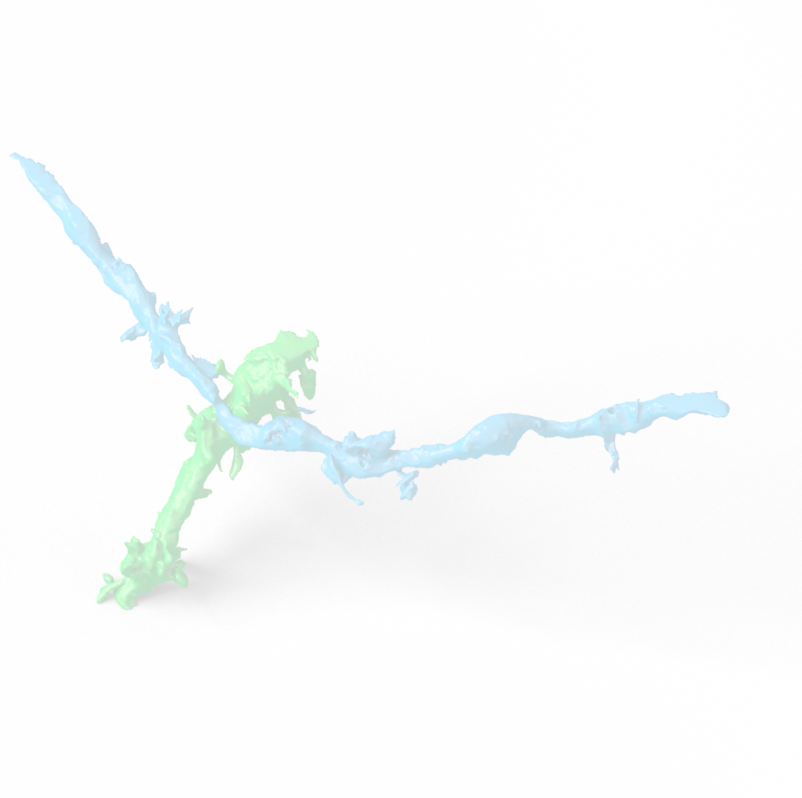
\includegraphics[width=440pt,height=440pt]{r0_watermark_25}
};
\end{tikzpicture}

\begin{textblock}{50}(140,200)
\color{date}\fontspec[Path = fonts/raleway/]{Raleway-ExtraLight}\fontsize{8pt}{10pt}\selectfont 
Ray-tracing of $100\mu m$-long neural processes captured at $4nm$ resolution.
\end{textblock}

\end{document}  \documentclass[]{article}
